\subsection{Resultados Punto 5: Constelación mediante Tabla de Verdad}

A partir de la metodología establecida, se analizó el comportamiento de la modulación 8-PSK generando una secuencia determinística de símbolos (del 0 al 7) utilizando una fuente de prueba controlada. Esto permitió validar la correspondencia exacta entre la tabla de verdad y la fase de la señal portadora en banda base.

En la Figura \ref{fig:constelacion_punto5} se presenta el diagrama de constelación resultante. Se observa que los símbolos se ubican de manera equidistante en el plano complejo, con una separación angular exacta de $\pi/4$ radianes entre cada punto adyacente. La ausencia de dispersión y la formación de un patrón circular perfecto confirman que la asignación estática del arreglo de números complejos se realizó correctamente, reflejando el ordenamiento natural esperado para este esquema M-PSK sin requerir procesamiento adicional.

\begin{figure}[htbp]
    \centering
    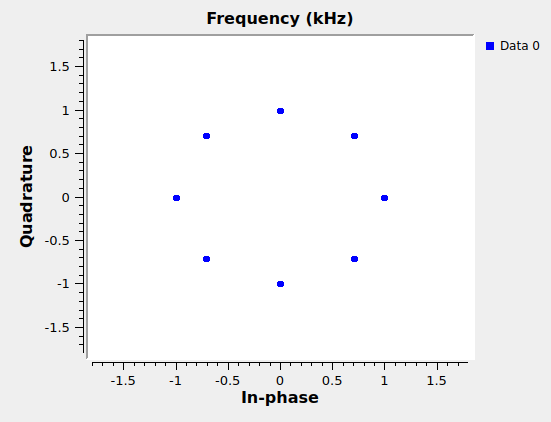
\includegraphics[width=0.6\linewidth]{imagenes/constelacion_punto5.png}
    \caption{Diagrama de constelación 8-PSK obtenido a partir de la tabla de verdad.}
    \label{fig:constelacion_punto5}
\end{figure}